\vspace{-6mm}
\section{Case Analysis and Qualitative Visualization}

In this section, we visualize the detection results of Grounding DINO 1.5 models in real-world scenarios. The images and text prompts are primarily sourced from the COCO~\cite{COCO}, LVIS~\cite{LVIS}, V3Det~\cite{V3Det}, OpenImages~\cite{OpenImages}, CC3M~\cite{CC12M} and SA-1B~\cite{SAM}. We are deeply grateful for their contributions, which have significantly benefited the community.


\subsection{Common Object Detection}
The visualizations presented in Figures \ref{fig:vis_common_obj} and \ref{fig:vis_common_obj2} demonstrate the robust performance of Grounding DINO 1.5 Pro for common object detection scenarios. Our model's proficiency is evident not only in its handling of typical cases but also in its ability to accurately detect objects under challenging conditions.

The model adeptly identifies objects in monochromatic images, where color cues are minimal, as illustrated by the first example in Figure \ref{fig:vis_common_obj}. This showcases the model's reliance on shape and texture to distinguish objects. The detection of blurry objects, as seen in the second example of Figure \ref{fig:vis_common_obj}, is a testament to the model's robustness against common image degradations, maintaining high accuracy even when visual clarity is compromised.

The ability to detect small and partially occluded objects is crucial for many applications. Grounding DINO 1.5 Pro's success in these scenarios, as shown in the last image in Figure \ref{fig:vis_common_obj}, indicates its fine-grained understanding and the nuanced integration of multi-modal information in autonomous driving scenes. The visualizations also highlight the model's versatility in handling objects of varying sizes and shapes, from petite to sprawling, each accurately localized and identified.

\begin{figure}[ht!]
\centering
 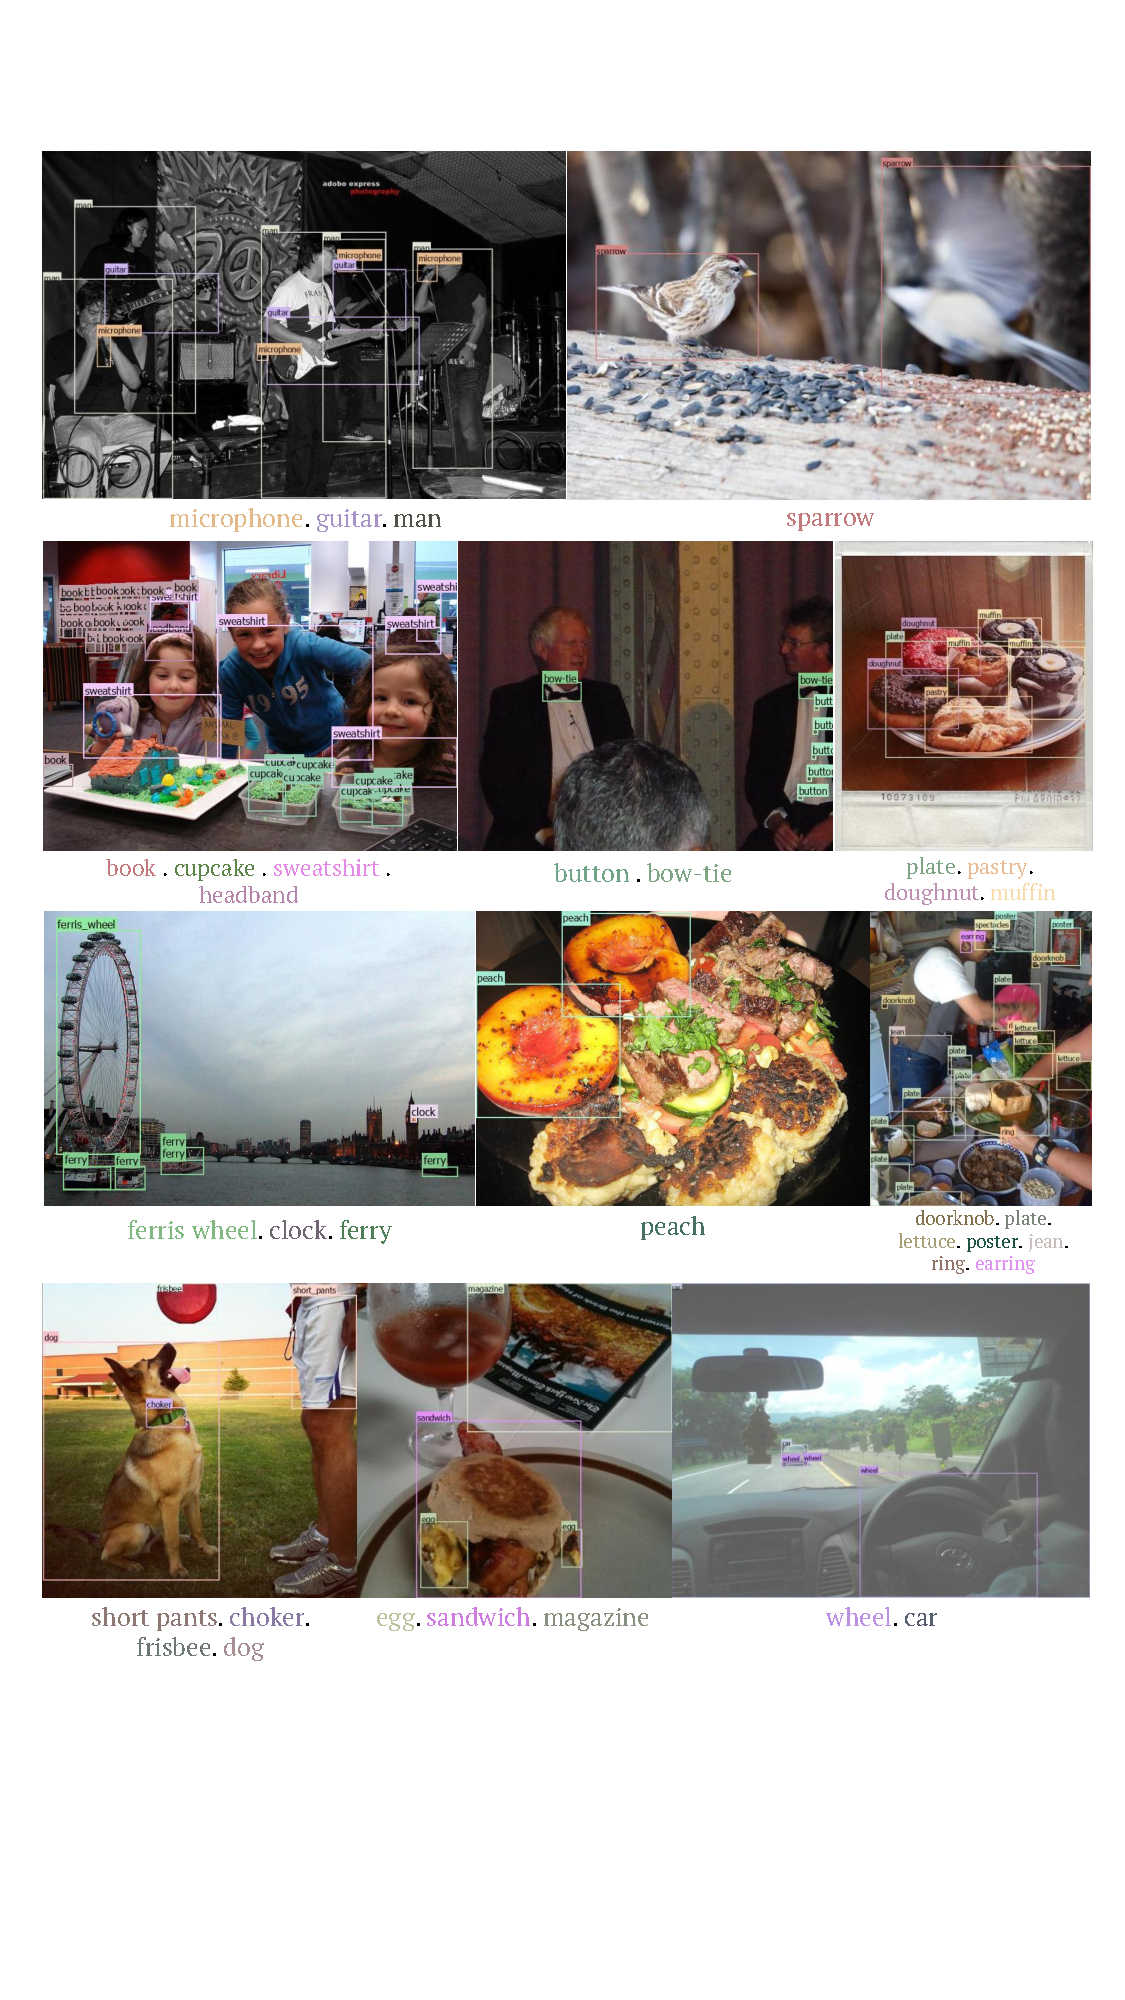
\includegraphics[width=1.0\textwidth,keepaspectratio]{figs/vis_v2/common_object_vis_v2.pdf}
 \caption{Model predictions on common objects with Grounding DINO 1.5 Pro (part 1).}
 \label{fig:vis_common_obj}
\end{figure}

\begin{figure}[ht!]
\centering
 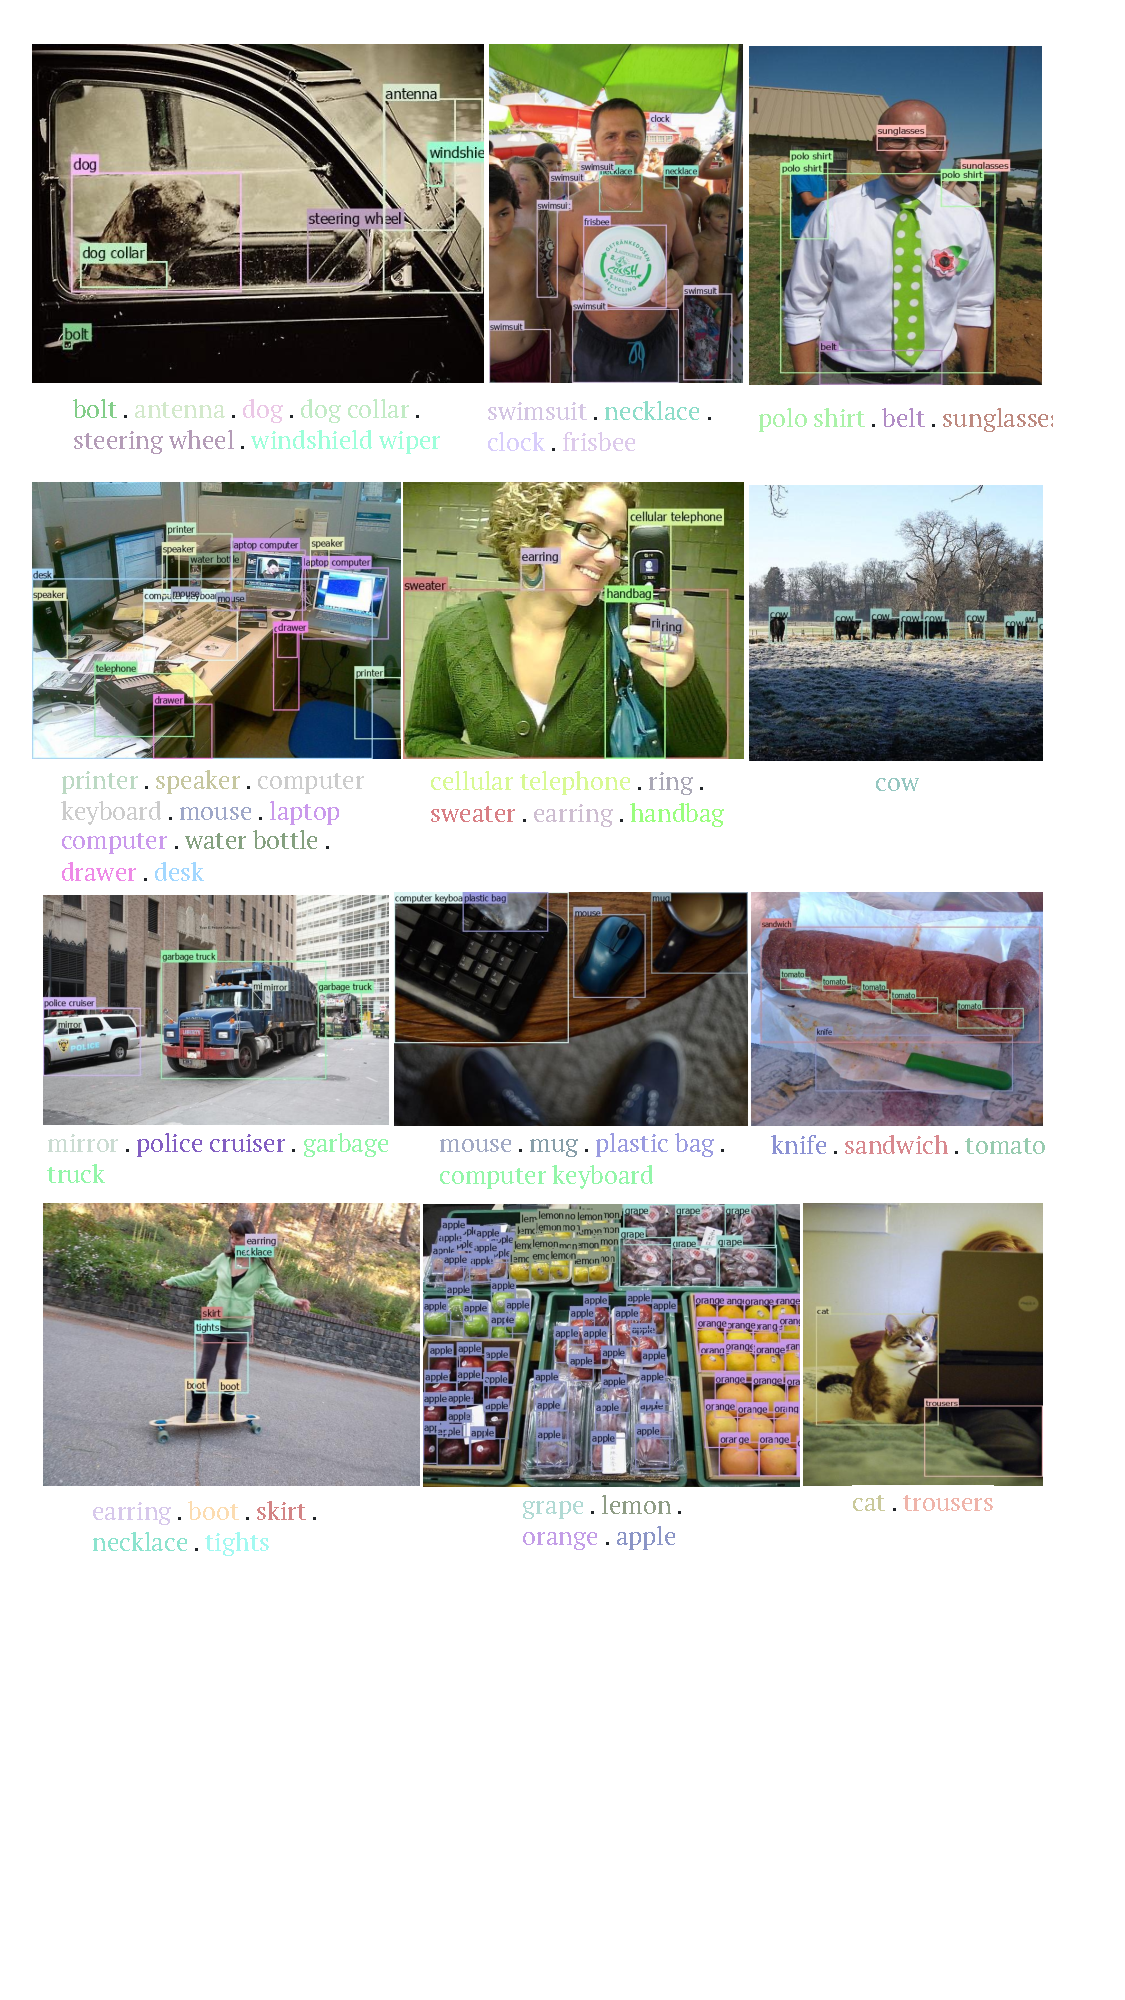
\includegraphics[width=1.0\textwidth,keepaspectratio]{figs/vis/common_object_vis2.pdf}
 \caption{Model predictions on common objects with Grounding DINO 1.5 Pro (part 2).}
 \label{fig:vis_common_obj2}
\end{figure}


\subsection{Long-tailed Object Detection}

This subsection delves into the capability of Grounding DINO 1.5 Pro in detecting long-tailed objects, which are less frequently encountered categories that pose unique challenges for object detection models. The examples provided in Figure \ref{fig:vis_long_tail} highlight the model's nuanced capability of understanding and detecting such uncommon objects. The model demonstrates its ability to recognize a diverse set of objects, including those that are not commonly found in everyday settings. 

For instance, the second image within the figure illustrates the model's capacity to identify a fungus, which is a category that requires specialized knowledge to discern. The third image showcases the model's fine-grained detection capabilities, accurately pinpointing a popsicle amidst a variety of potential distractors. The model's contextual understanding is evident in its ability to detect a taco in the last image of the third line, an object that may be challenging to recognize without the appropriate contextual cues.



\begin{figure}[ht!]
\centering
 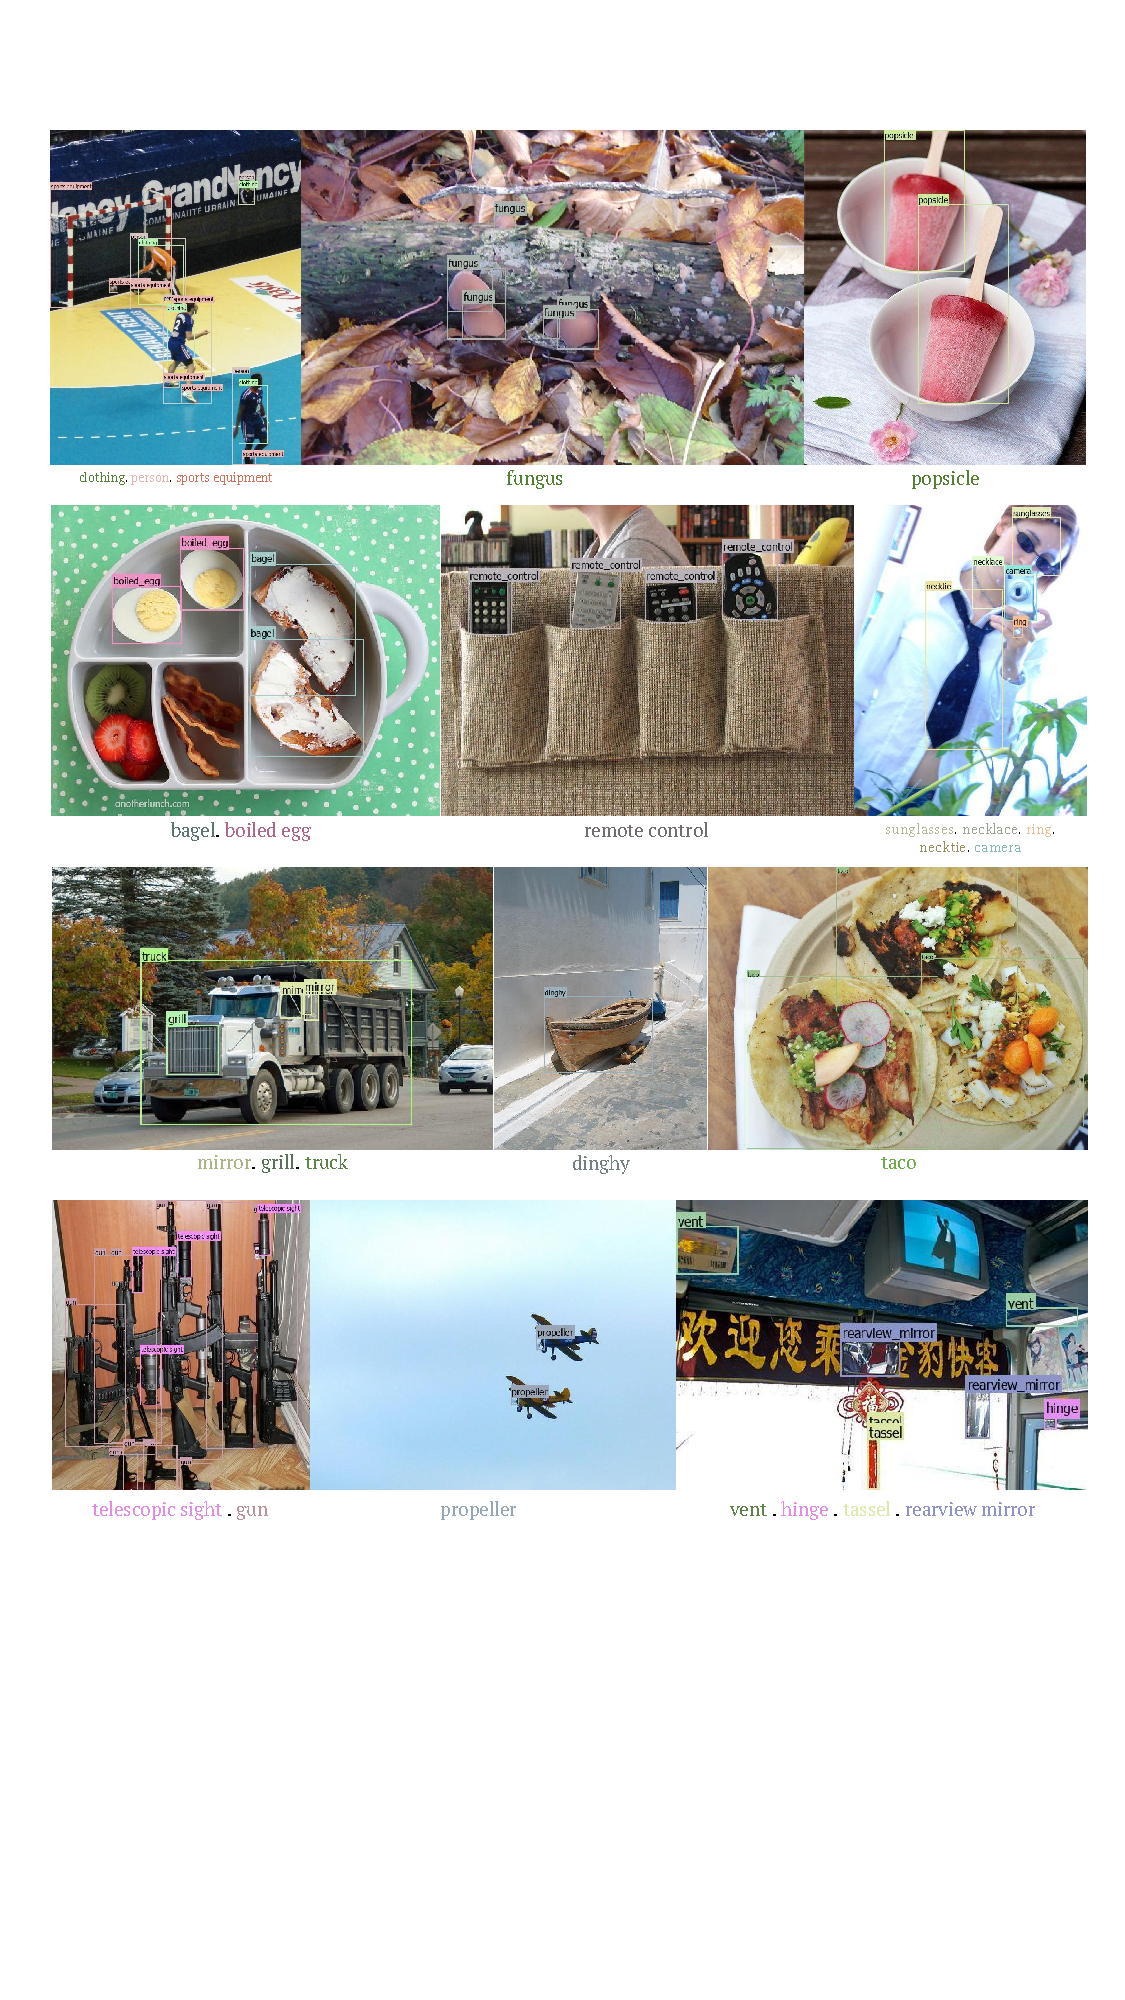
\includegraphics[width=\textwidth,keepaspectratio]{figs/vis/longtail_category.pdf}
 \caption{Model predictions on long-tailed categories with Grounding DINO 1.5 Pro.
}
 \label{fig:vis_long_tail}
\end{figure}




\subsection{Short Caption Grounding}

Grounding models can correlate objects within images to their corresponding mentions in accompanying captions. This capability is particularly significant for enhancing the contextual understanding of visual content across various domains. In Figure \ref{fig:vis_short_cap}, we present Grounding DINO 1.5 Pro's proficiency in short caption grounding, highlighting its versatility and accuracy.

The model exhibits a robust performance in grounding objects across different visual domains. It adeptly handles real-world images while also demonstrating a keen ability to interpret objects within cartoons, sketches, and animations. By aligning textual descriptions with visual features, the model can accurately identify and localize objects, even when they appear in stylized or abstract forms.


\begin{figure}[ht!]
\centering
 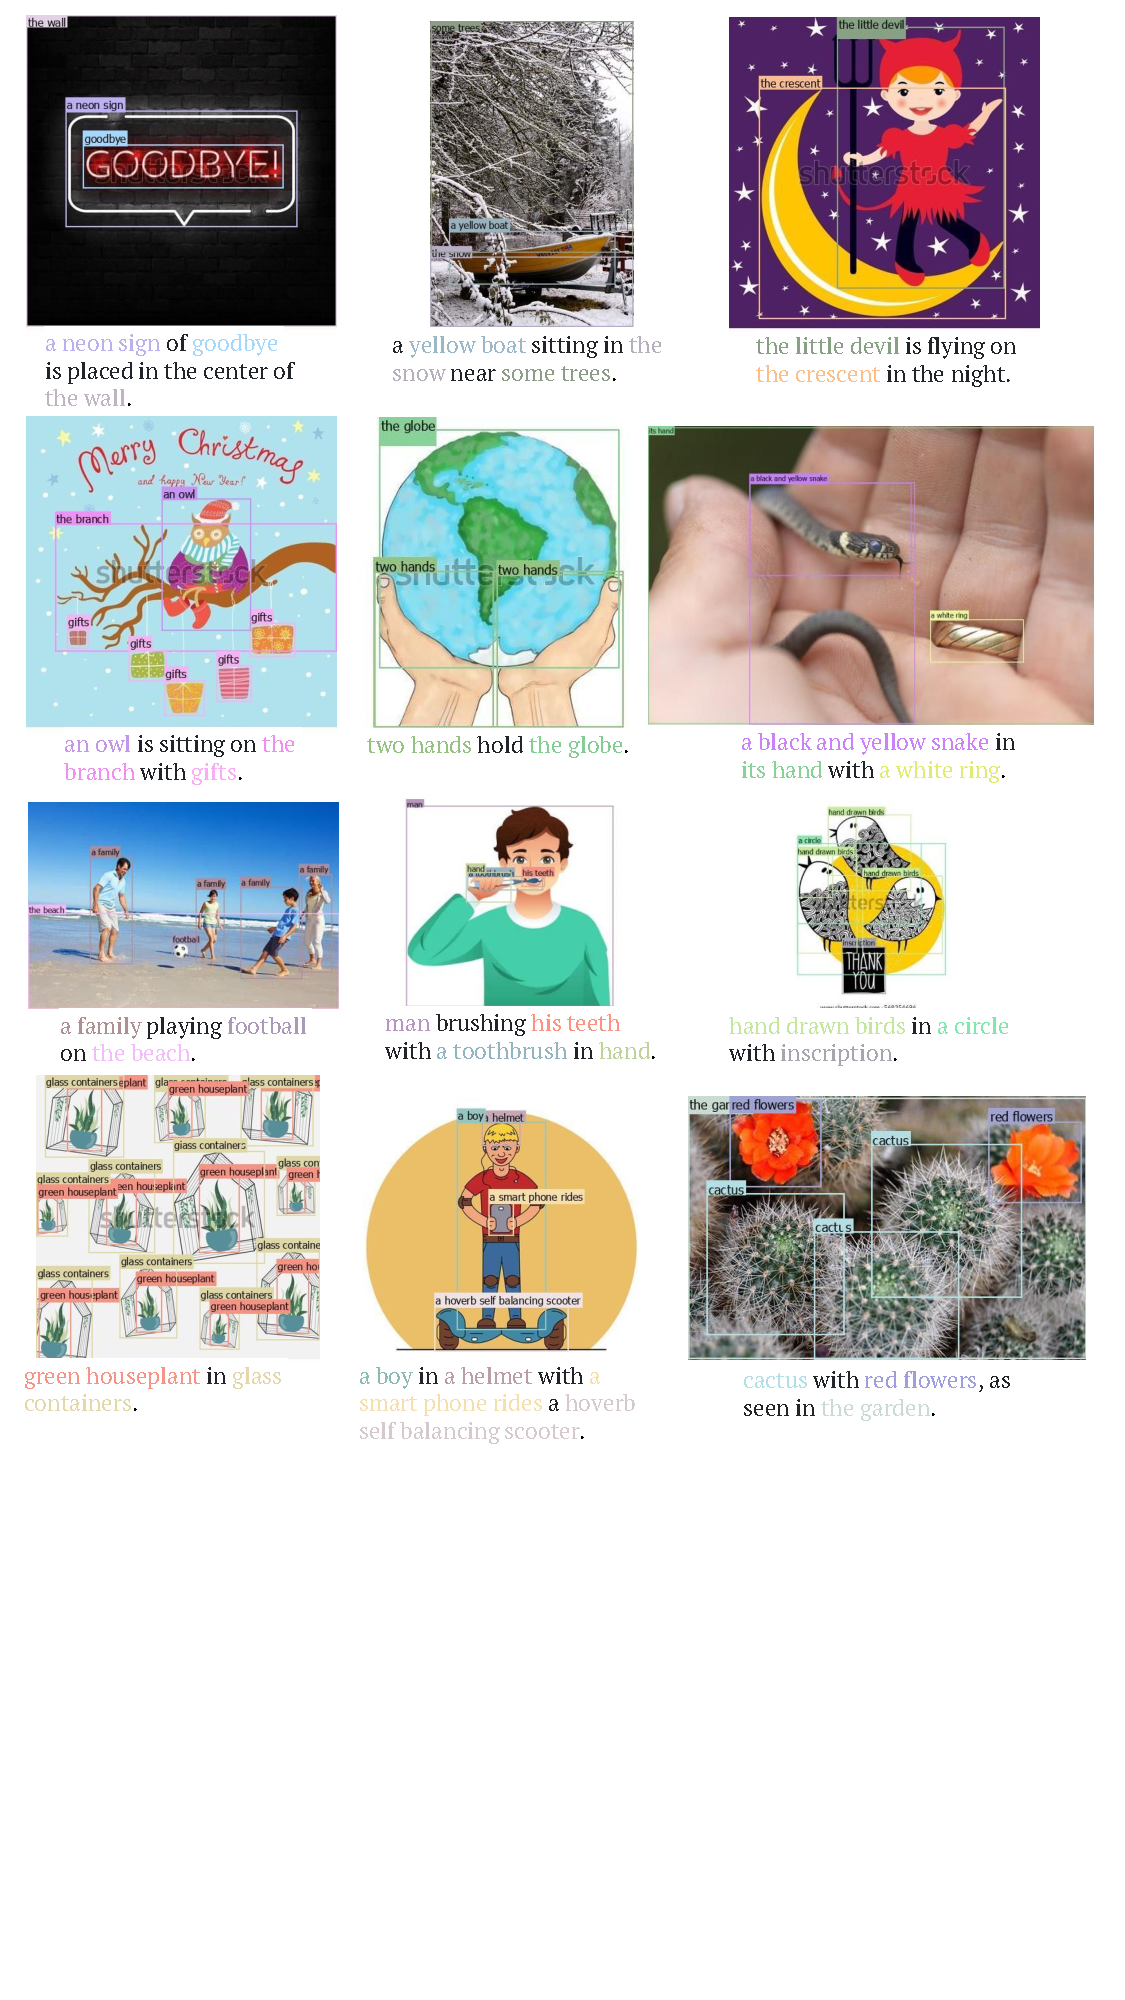
\includegraphics[width=0.92\textwidth,keepaspectratio]{figs/vis_v2/short_caption_vis_v3.pdf}
 \caption{Phrase grounding on short captions with Grounding DINO 1.5 Pro.
}
 \label{fig:vis_short_cap}
\end{figure}


\subsection{Long Caption Grounding}

Our model, Grounding DINO 1.5 Pro, extends its capability beyond the realm of standard image-caption pairs to adeptly handle long captions, as depicted in Figure \ref{fig:vis_long_cap1}, Figure \ref{fig:vis_long_cap2} and Figure \ref{fig:vis_long_cap3}. Long captions offer a richer tapestry of details that can more comprehensively describe the visual content of an image. The ability to map each noun phrase in a long caption to corresponding objects within an image is a significant step toward deeper image understanding.

An intriguing observation is the model's ability to generalize from pre-training on captions with shorter context windows to effectively processing longer contexts. This adaptability suggests that larger models may inherently possess flexibility that can be leveraged for various lengths of textual input.

Grounding DINO 1.5 Pro exhibits an impressive capacity to correlate textual phrases with visual elements. This capability is not only showcased in the model's handling of long captions but also in its nuanced analysis of images at multiple granularities. Moreover, we notice that the model can detect some terms that did not show in the training data, like \texttt{fiat logo} in the third image. It presents the strong generalization ability of the model. 



\begin{figure}[ht!]
\centering
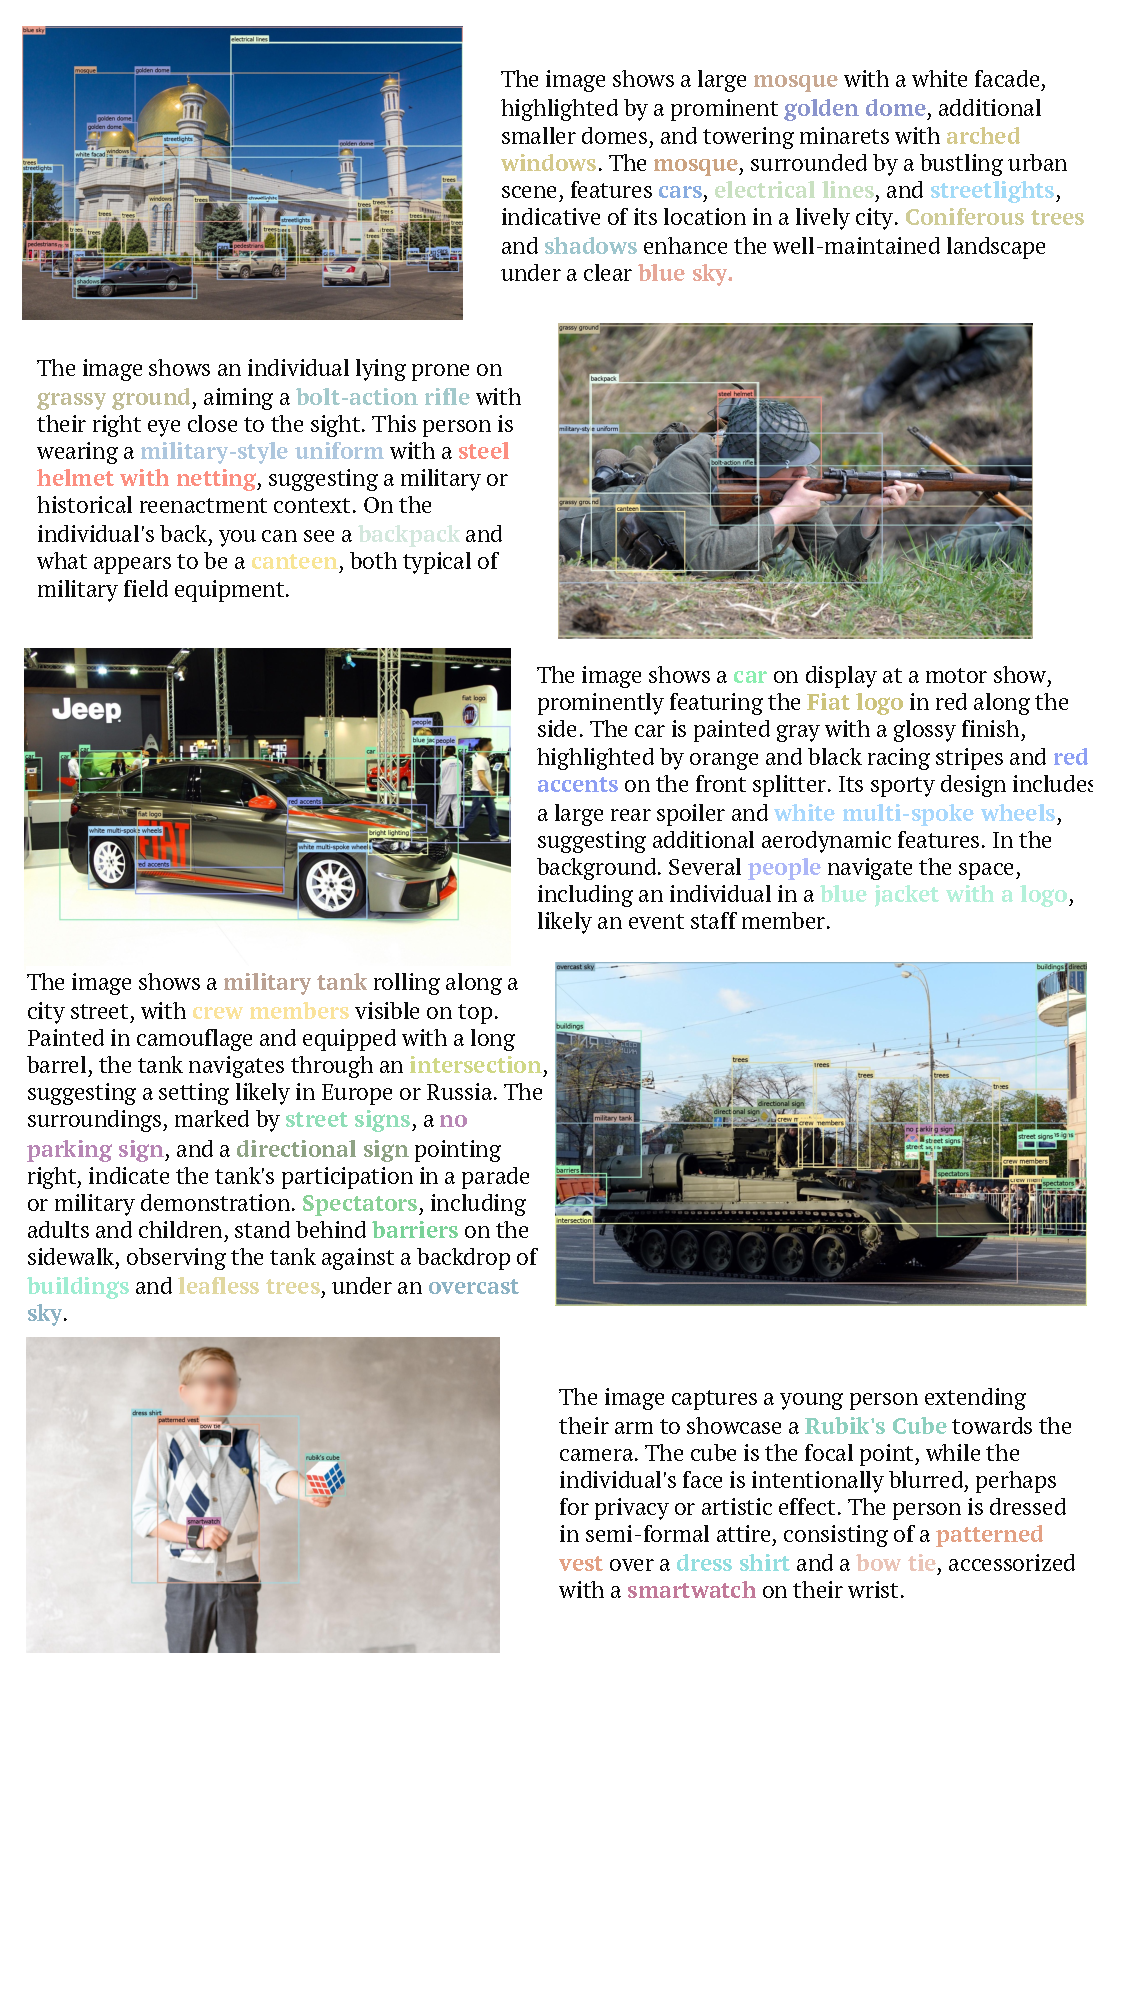
\includegraphics[width=1.0\textwidth,keepaspectratio]{figs/vis/long_caption_vis.pdf}
 \caption{Phrase grounding on long captions with Grounding DINO 1.5 Pro (part 1).
}
 \label{fig:vis_long_cap1}
\end{figure}

\begin{figure}[ht!]
\centering
 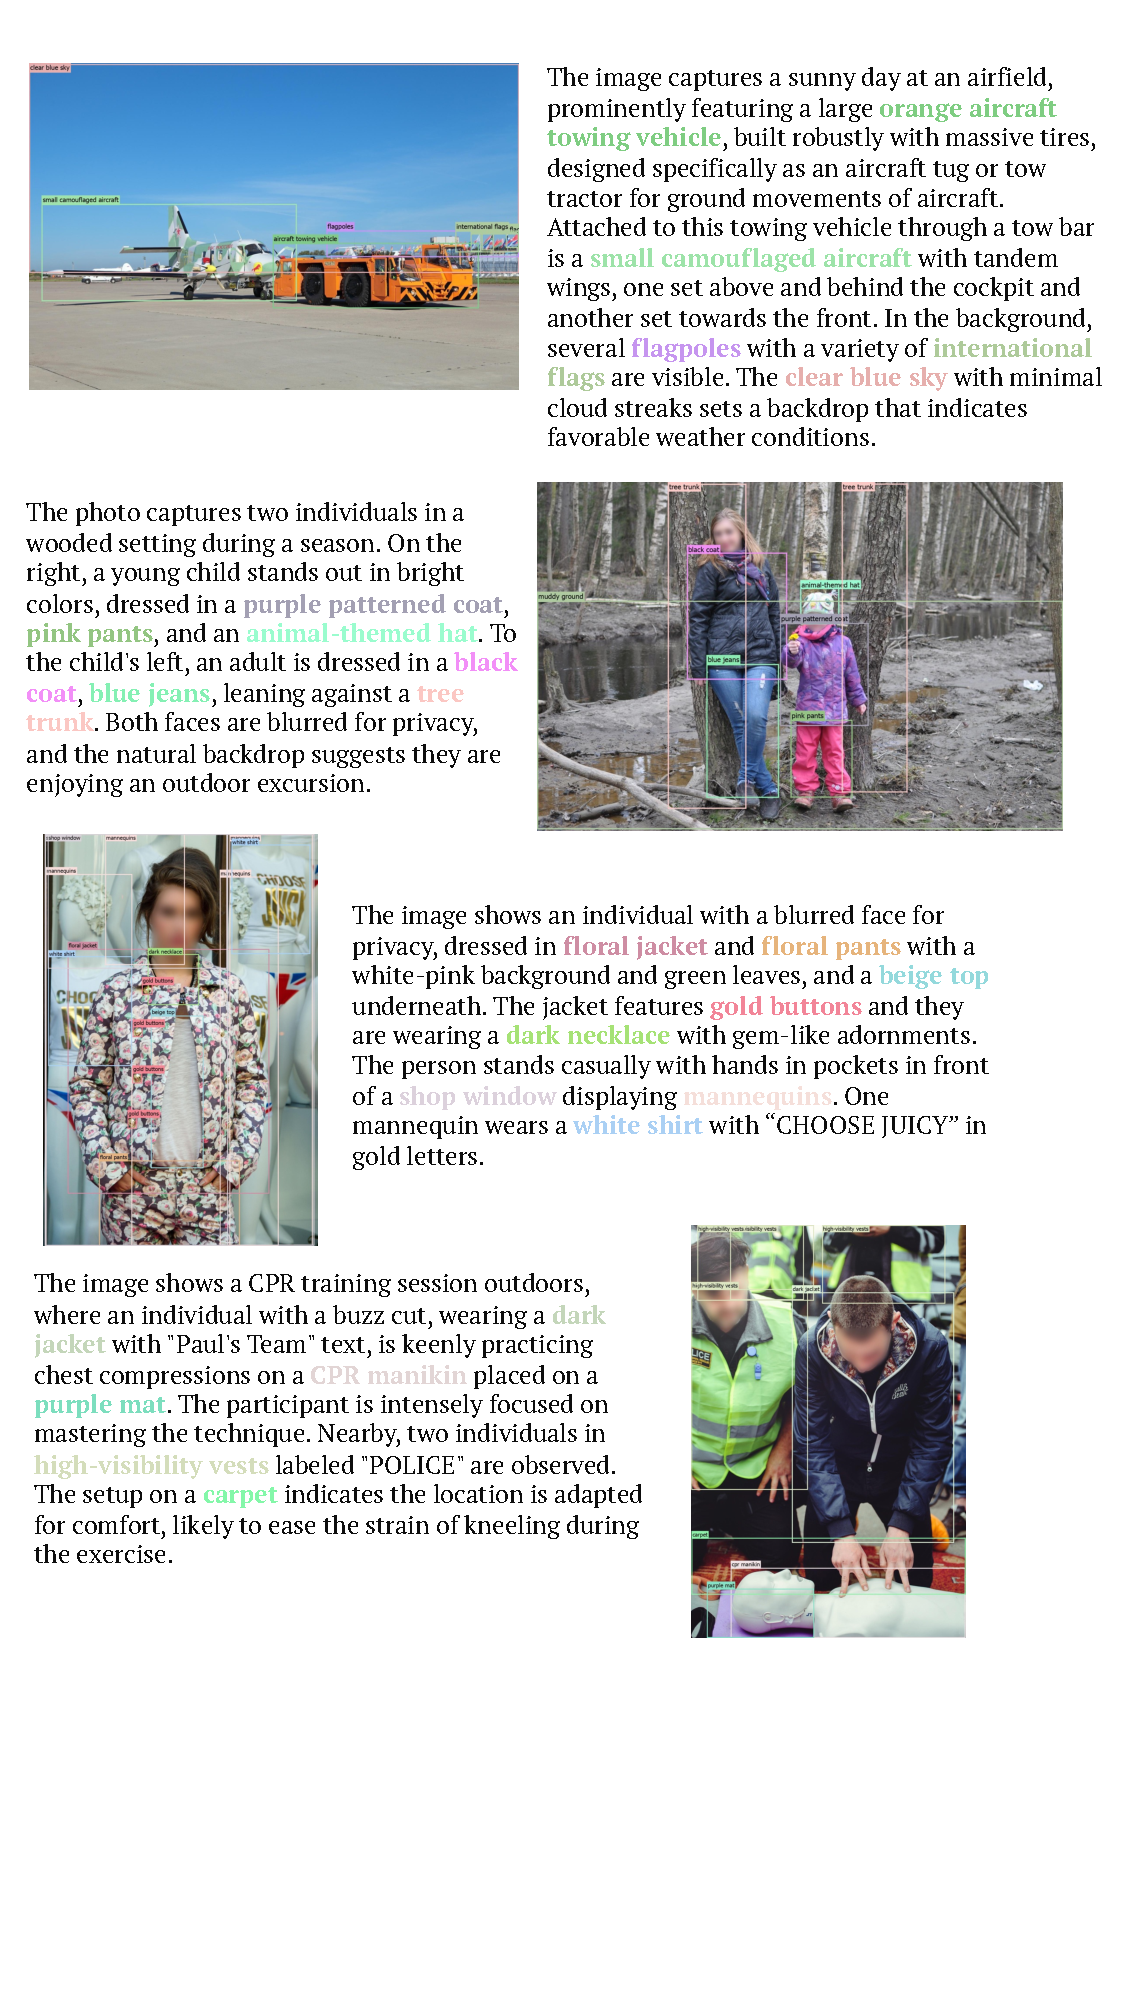
\includegraphics[width=0.98\textwidth,keepaspectratio]{figs/vis/long_caption_vis2.pdf}
 \caption{Phrase grounding on long captions with Grounding DINO 1.5 Pro (part 2). 
}
 \label{fig:vis_long_cap2}
\end{figure}

\begin{figure}[ht!]
\centering
 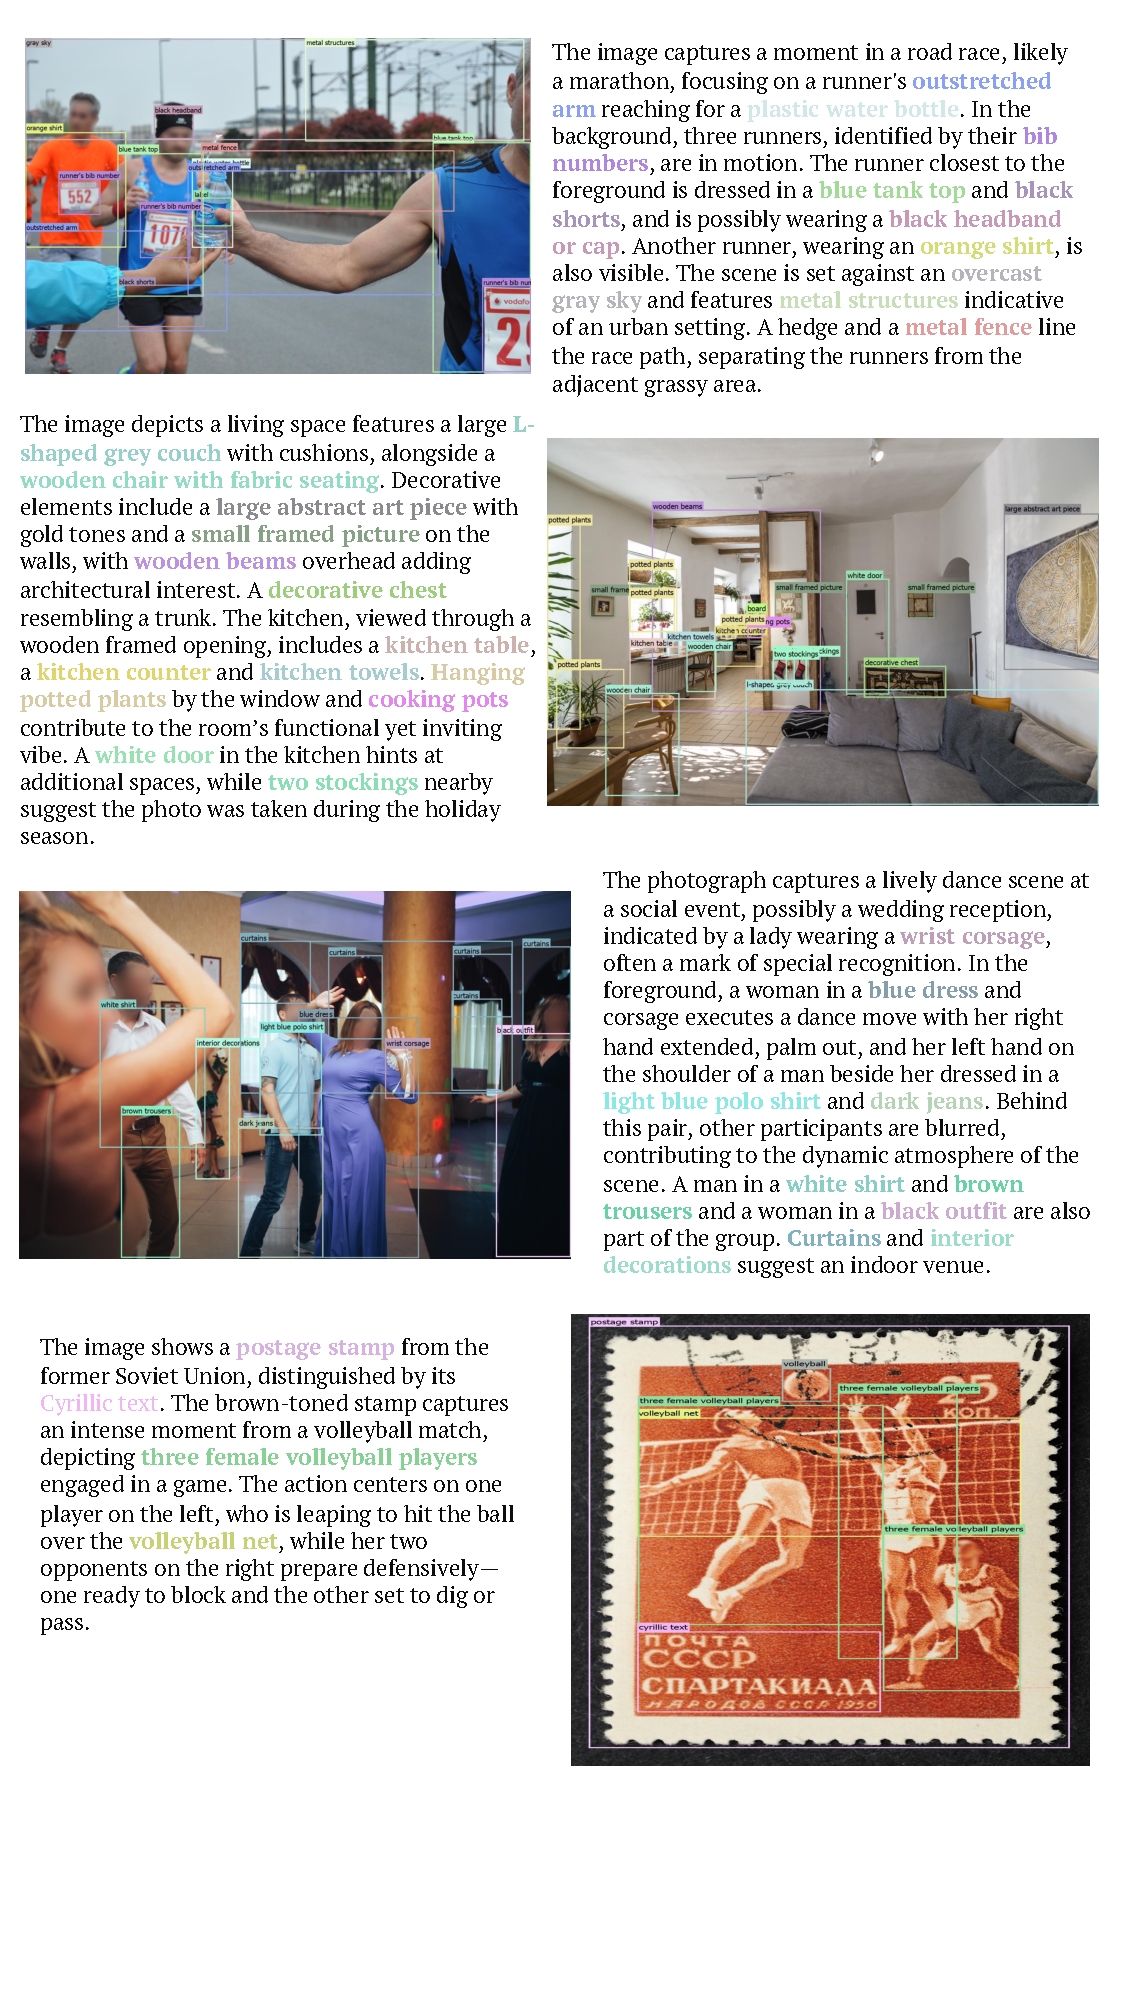
\includegraphics[width=0.98\textwidth,keepaspectratio]{figs/vis/long_caption_vis3.pdf}
 \caption{Phrase grounding on long captions with Grounding DINO 1.5 Pro (part 3).
}
 \label{fig:vis_long_cap3}
\end{figure}


\subsection{Dense Object Detection}

Grounding DINO 1.5 Pro showcases an exceptional capability to discern objects within dense scenarios, where multiple objects are closely positioned or overlapping, making detection a challenging task. This ability is vividly demonstrated through the visualizations presented in Figure \ref{fig:vis_dense_obj} and Figure \ref{fig:vis_dense_obj2}.

The model's performance is noteworthy across a wide spectrum of object nomenclature. It adeptly identifies objects labeled with common names such as \texttt{coin}, \texttt{tree}, \texttt{flower}, and \texttt{land}. Moreover, the model also excels at recognizing objects denoted by specialized terminology, including \texttt{kohlrabi}, \texttt{atlantic puffin}, and \texttt{oxalis purpurea}. 


\begin{figure}[ht!]
 \centering
 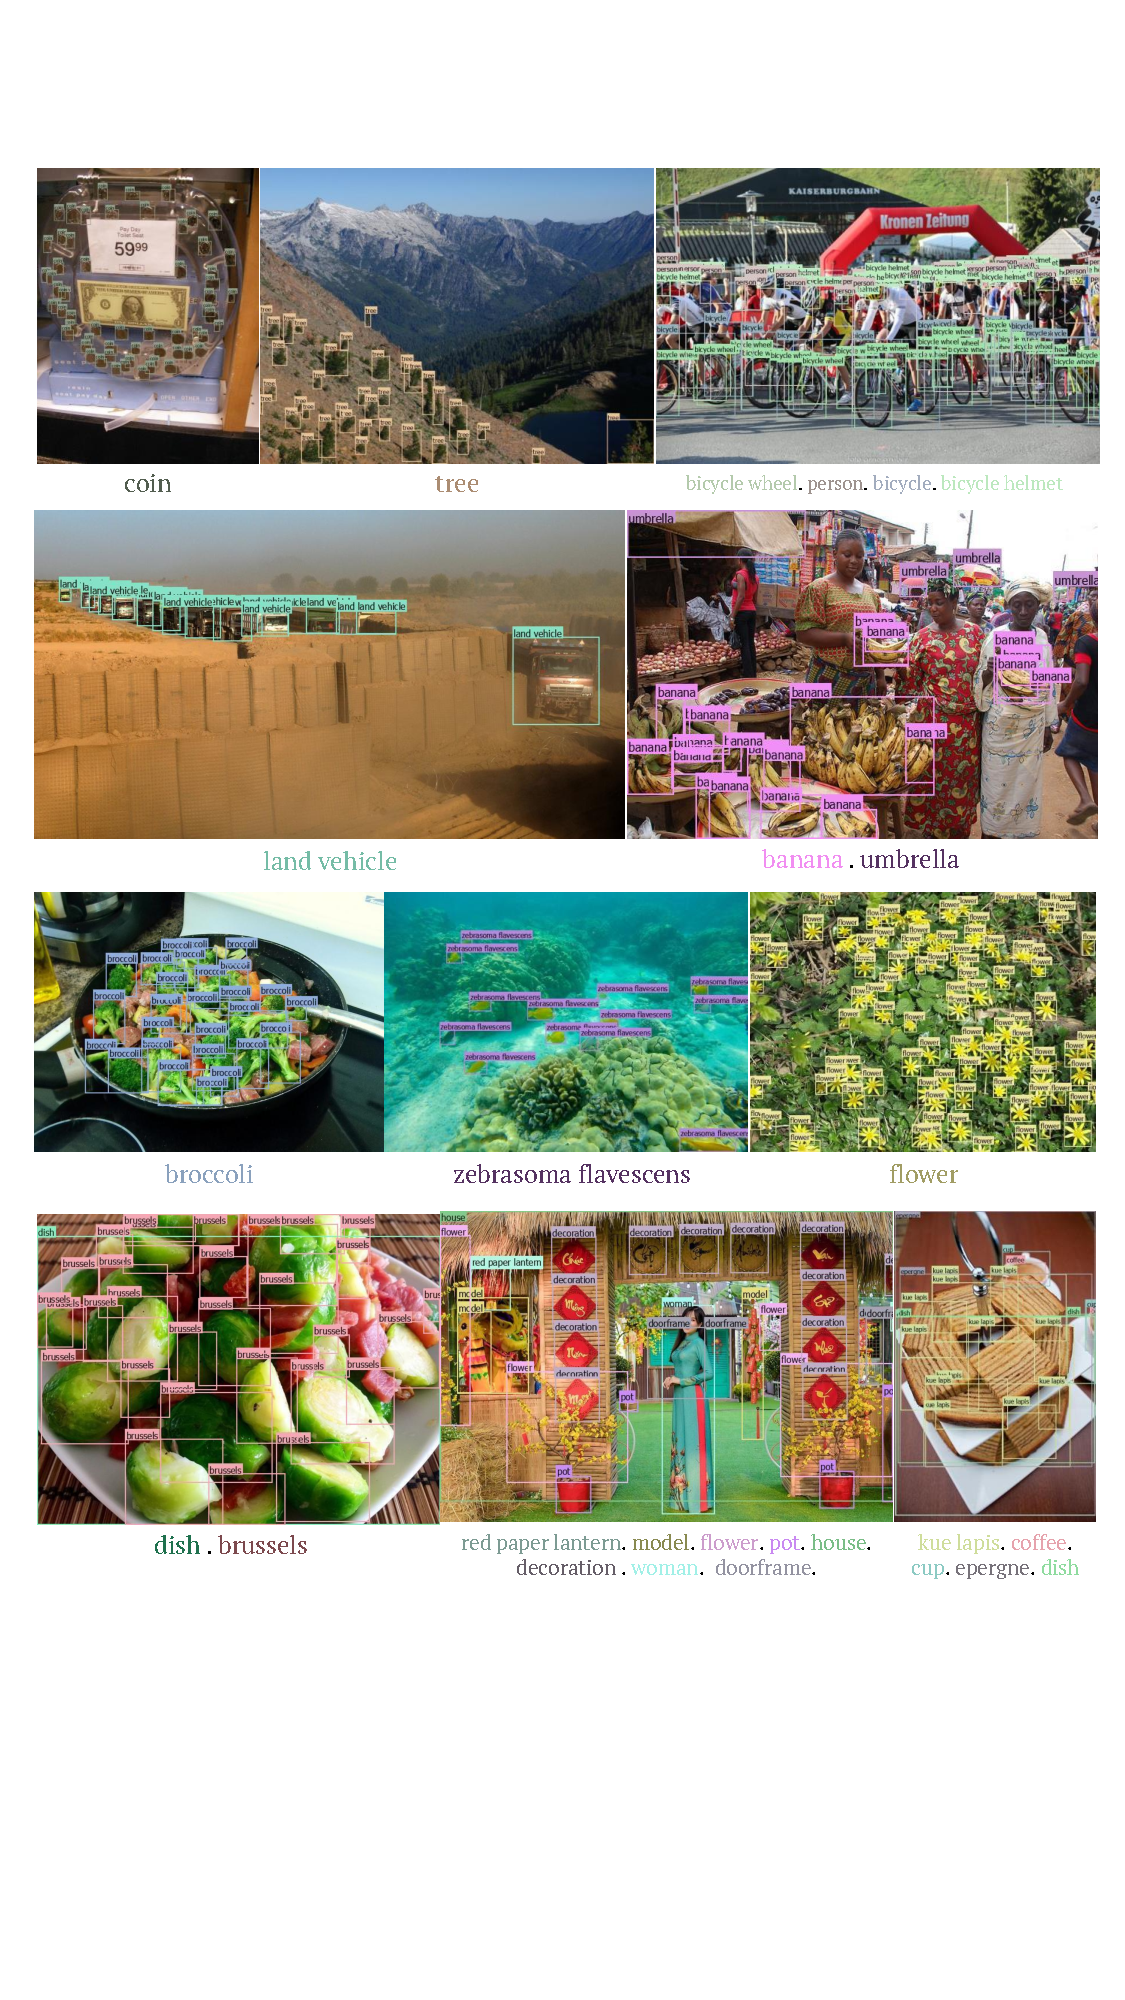
\includegraphics[width=1.0\textwidth,keepaspectratio]{figs/vis_v2/dense_object_vis_v3.pdf}
 \caption{Model predictions on dense object scenarios with Grounding DINO 1.5 Pro (part 1).
}
 \label{fig:vis_dense_obj}
\end{figure}

\begin{figure}[ht!]
\centering
 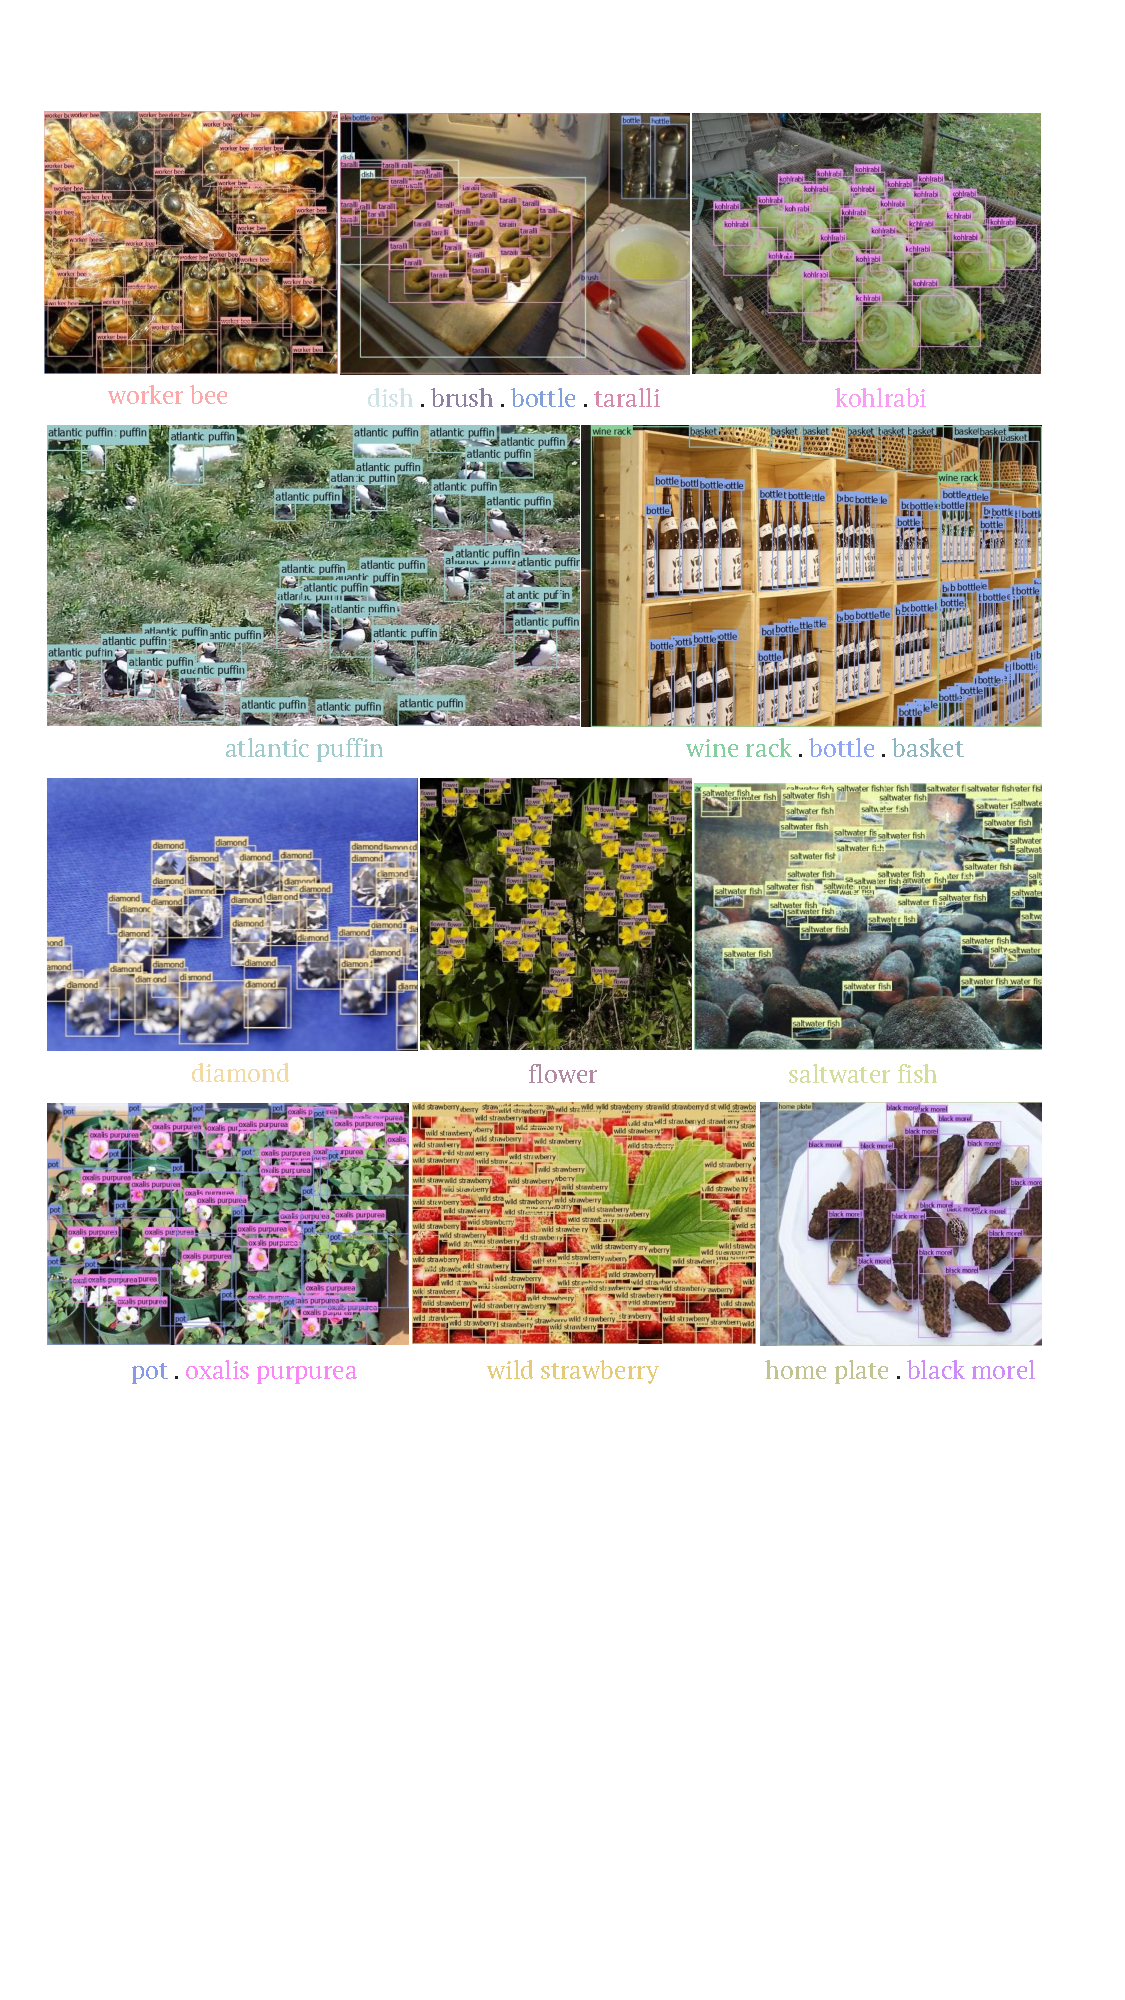
\includegraphics[width=\textwidth,keepaspectratio]{figs/vis_v2/dense_object_vis2_v2.pdf}
 \caption{Model predictions on dense object scenarios with Grounding DINO 1.5 Pro (part 2).
}
 \label{fig:vis_dense_obj2}
\end{figure}


\subsection{Video Object Detection}

We present video detection results of Grounding DINO 1.5 Pro in Figure \ref{fig:video_vis}. We notice the model can produce consistent object bounding boxes in most cases. The videos are processed offline.

\begin{figure}[ht!]
\centering
 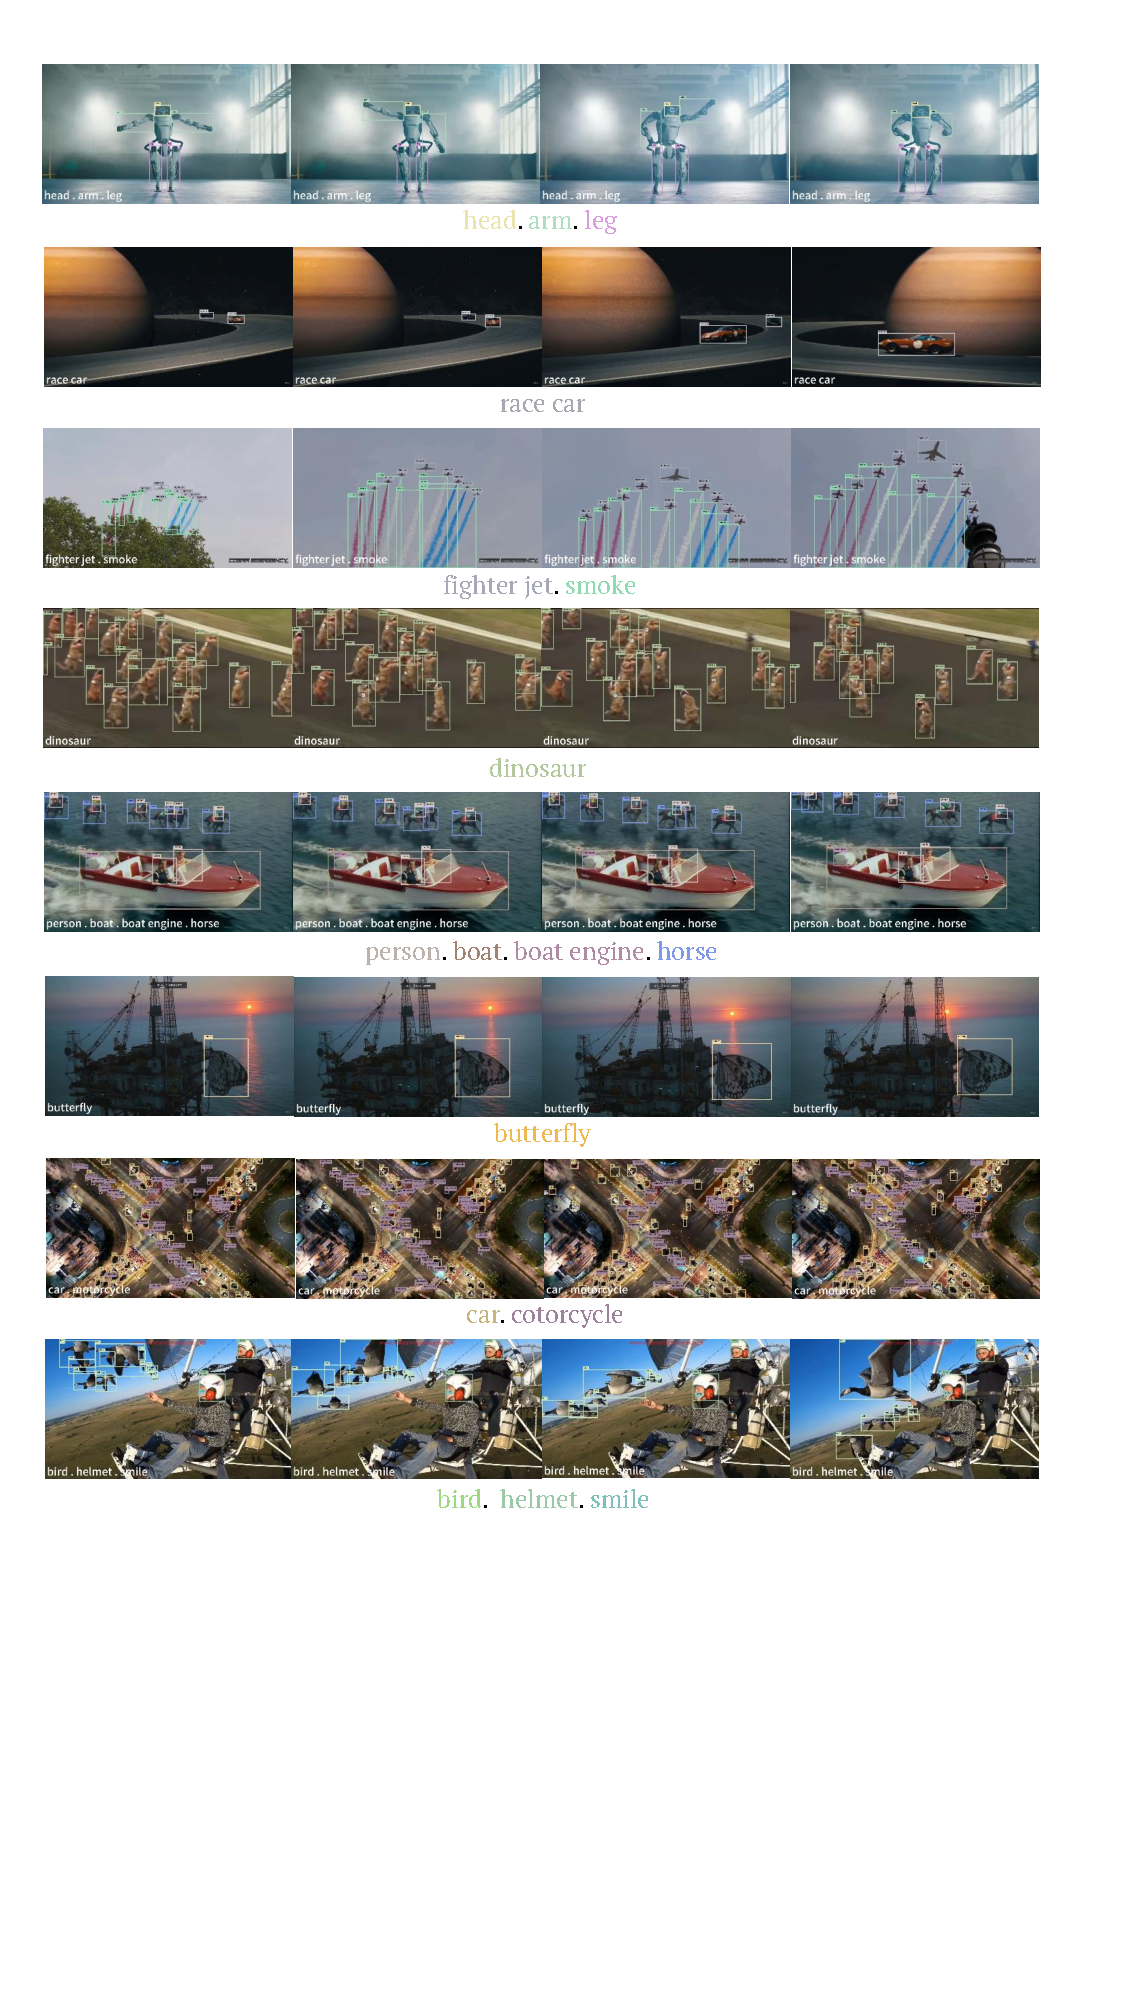
\includegraphics[width=1.0\textwidth,keepaspectratio]{figs/vis_v2/video_object_vis_v2.pdf}
 \caption{Model predictions on video object detection with Grounding DINO 1.5 Pro.
}
 \label{fig:video_vis}
\end{figure}


\subsection{Side-by-side Comparison}

We present the side-by-side comparison between the results of Grounding DINO 1.5 Pro and Grounding DINO in Figure \ref{fig:side_by_side_compare_part1} and Figure \ref{fig:side_by_side_compare_part2}. The Grounding DINO 1.5 Pro model demonstrates superior performance over the Grounding DINO model in terms of dense scene detection, long-tailed object detection, and the accuracy of semantic understanding.


Moreover, we compare the object hallucinations of Grounding DINO 1.5 Pro and Grounding DINO, as shown in Figure \ref{fig:vis_halluci}. The results show that Grounding DINO 1.5 Pro has better accuracy and fewer object hallucinations. The last line in Figure \ref{fig:vis_halluci} demonstrates the better context understanding ability of our model.



\begin{figure}[ht!]
\centering
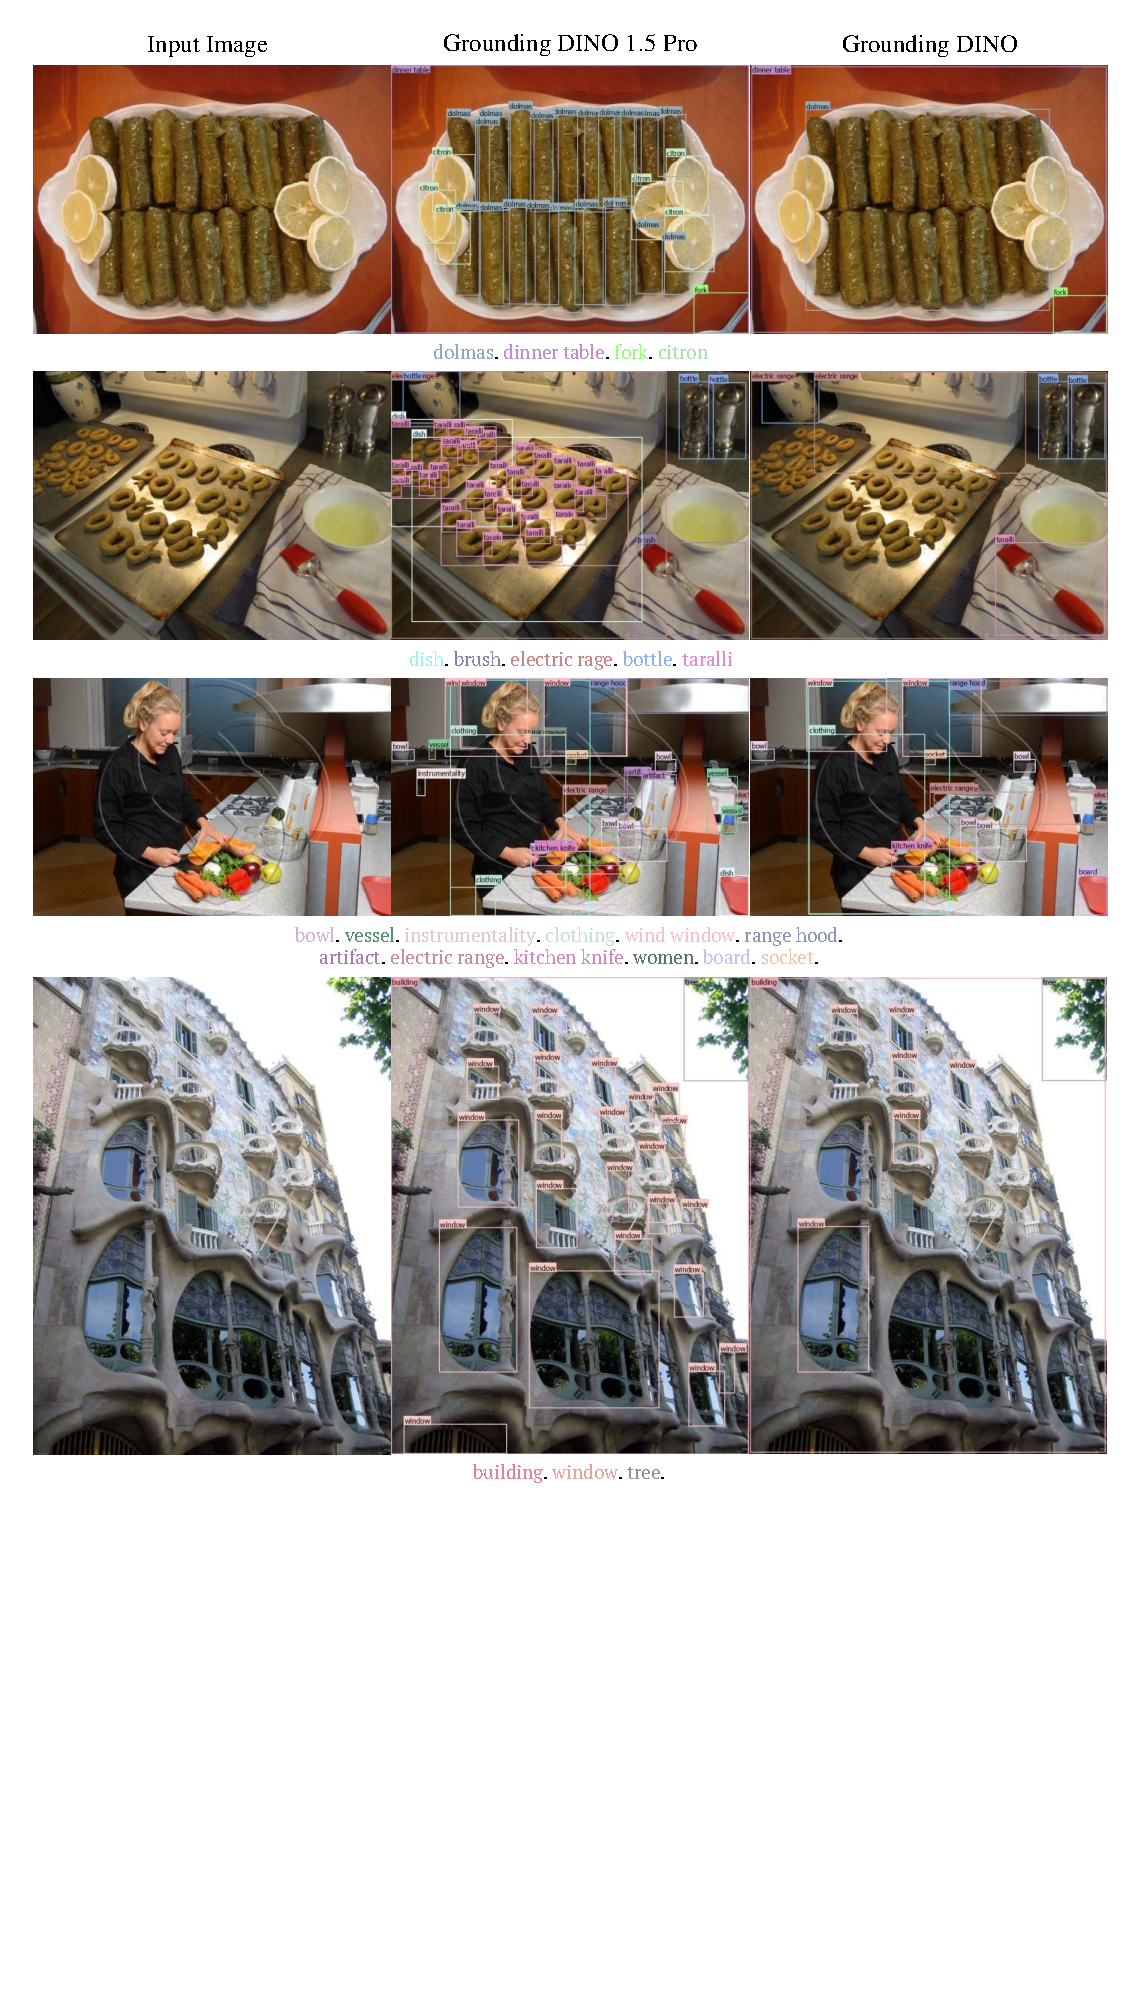
\includegraphics[width=\textwidth,keepaspectratio]{figs/vis/gd_1.5_vs_1.0_part1.pdf}
 \caption{Side-by-side comparison between Grounding DINO 1.5 Pro and Grounding DINO~\cite{GroundingDINO} (part 1).
}
 \label{fig:side_by_side_compare_part1}
\end{figure}

\begin{figure}[ht!]
\centering
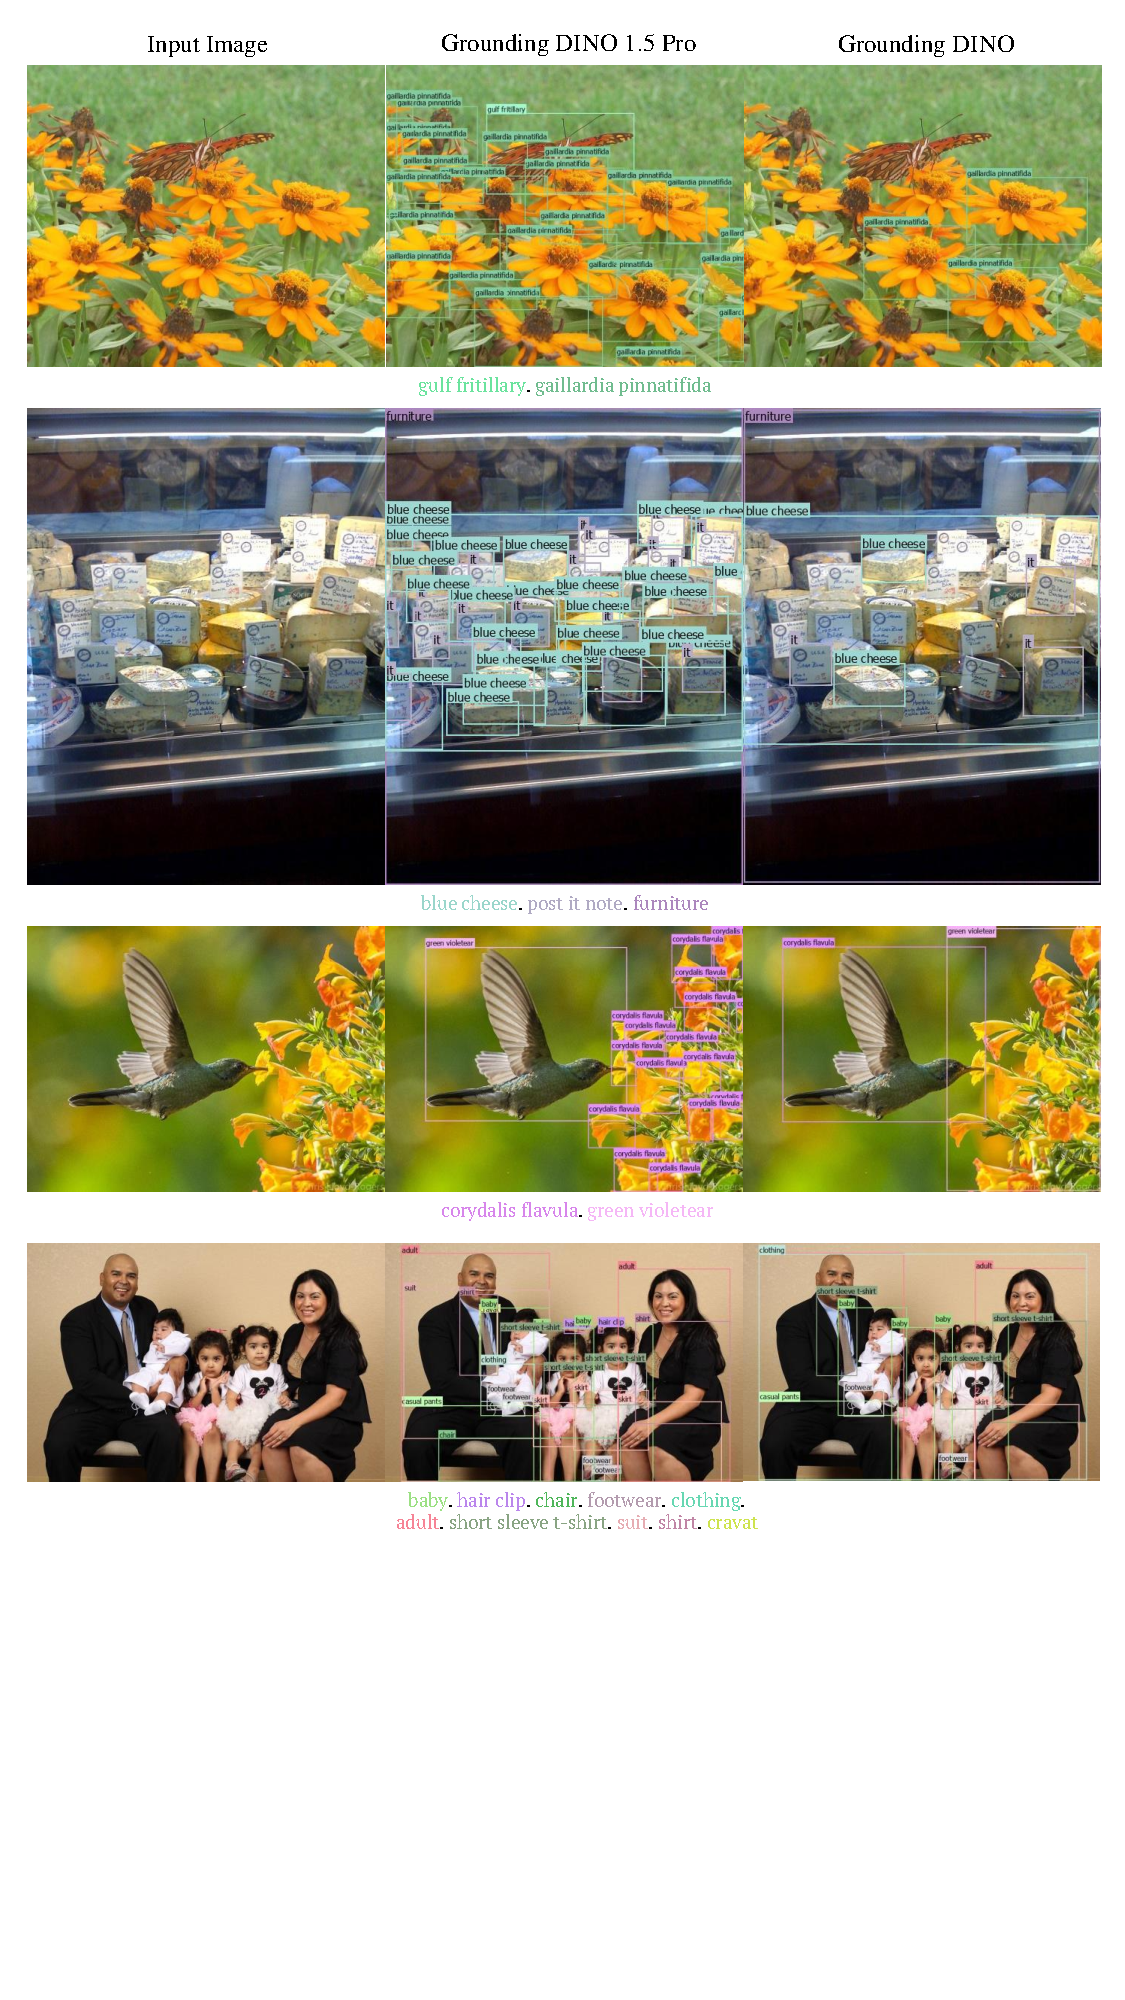
\includegraphics[width=\textwidth,keepaspectratio]{figs/vis/gd_1.5_vs_1.0_part2.pdf}
 \caption{Side-by-side comparison between Grounding DINO 1.5 Pro and Grounding DINO~\cite{GroundingDINO} (part 2).
}
 \label{fig:side_by_side_compare_part2}
\end{figure}



\begin{figure}[ht!]
\centering
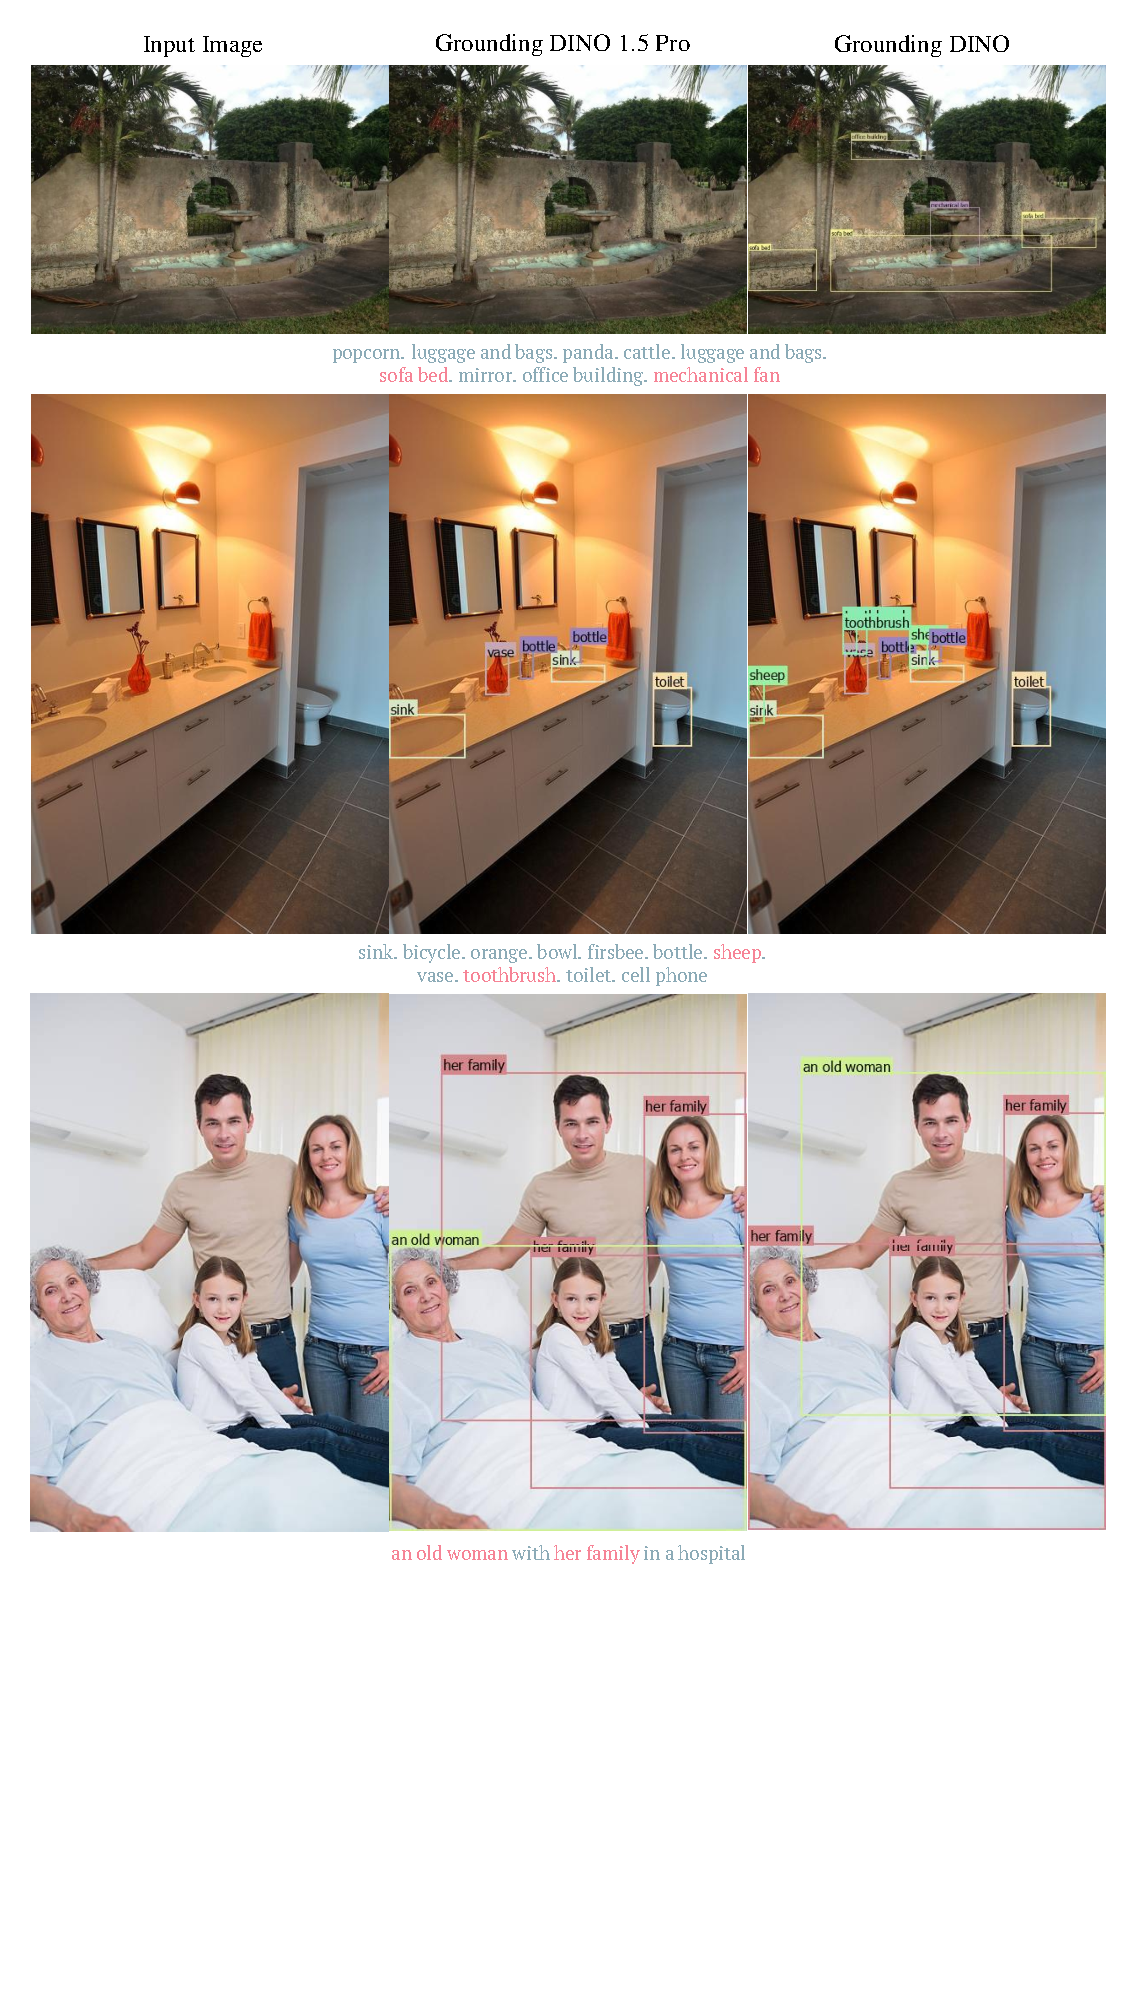
\includegraphics[width=\textwidth,keepaspectratio]{figs/vis_v2/hallucination_gd1.5_vs_gd1.pdf}
 \caption{Side-by-side comparison between Grounding DINO 1.5 Pro and Grounding DINO~\cite{GroundingDINO} regarding object hallucinations. 
}
 \label{fig:vis_halluci}
\end{figure}





\subsection{Advanced Object Detection on Edge Devices}

We present the practical, real-time application potential of Grounding DINO 1.5 Edge through a series of demonstrations in Figure \ref{fig:edge_vis}. The model's adept performance in office environments is particularly highlighted, offering significant utility for the field of robotics research.


\begin{figure}[t!]
    \centering
    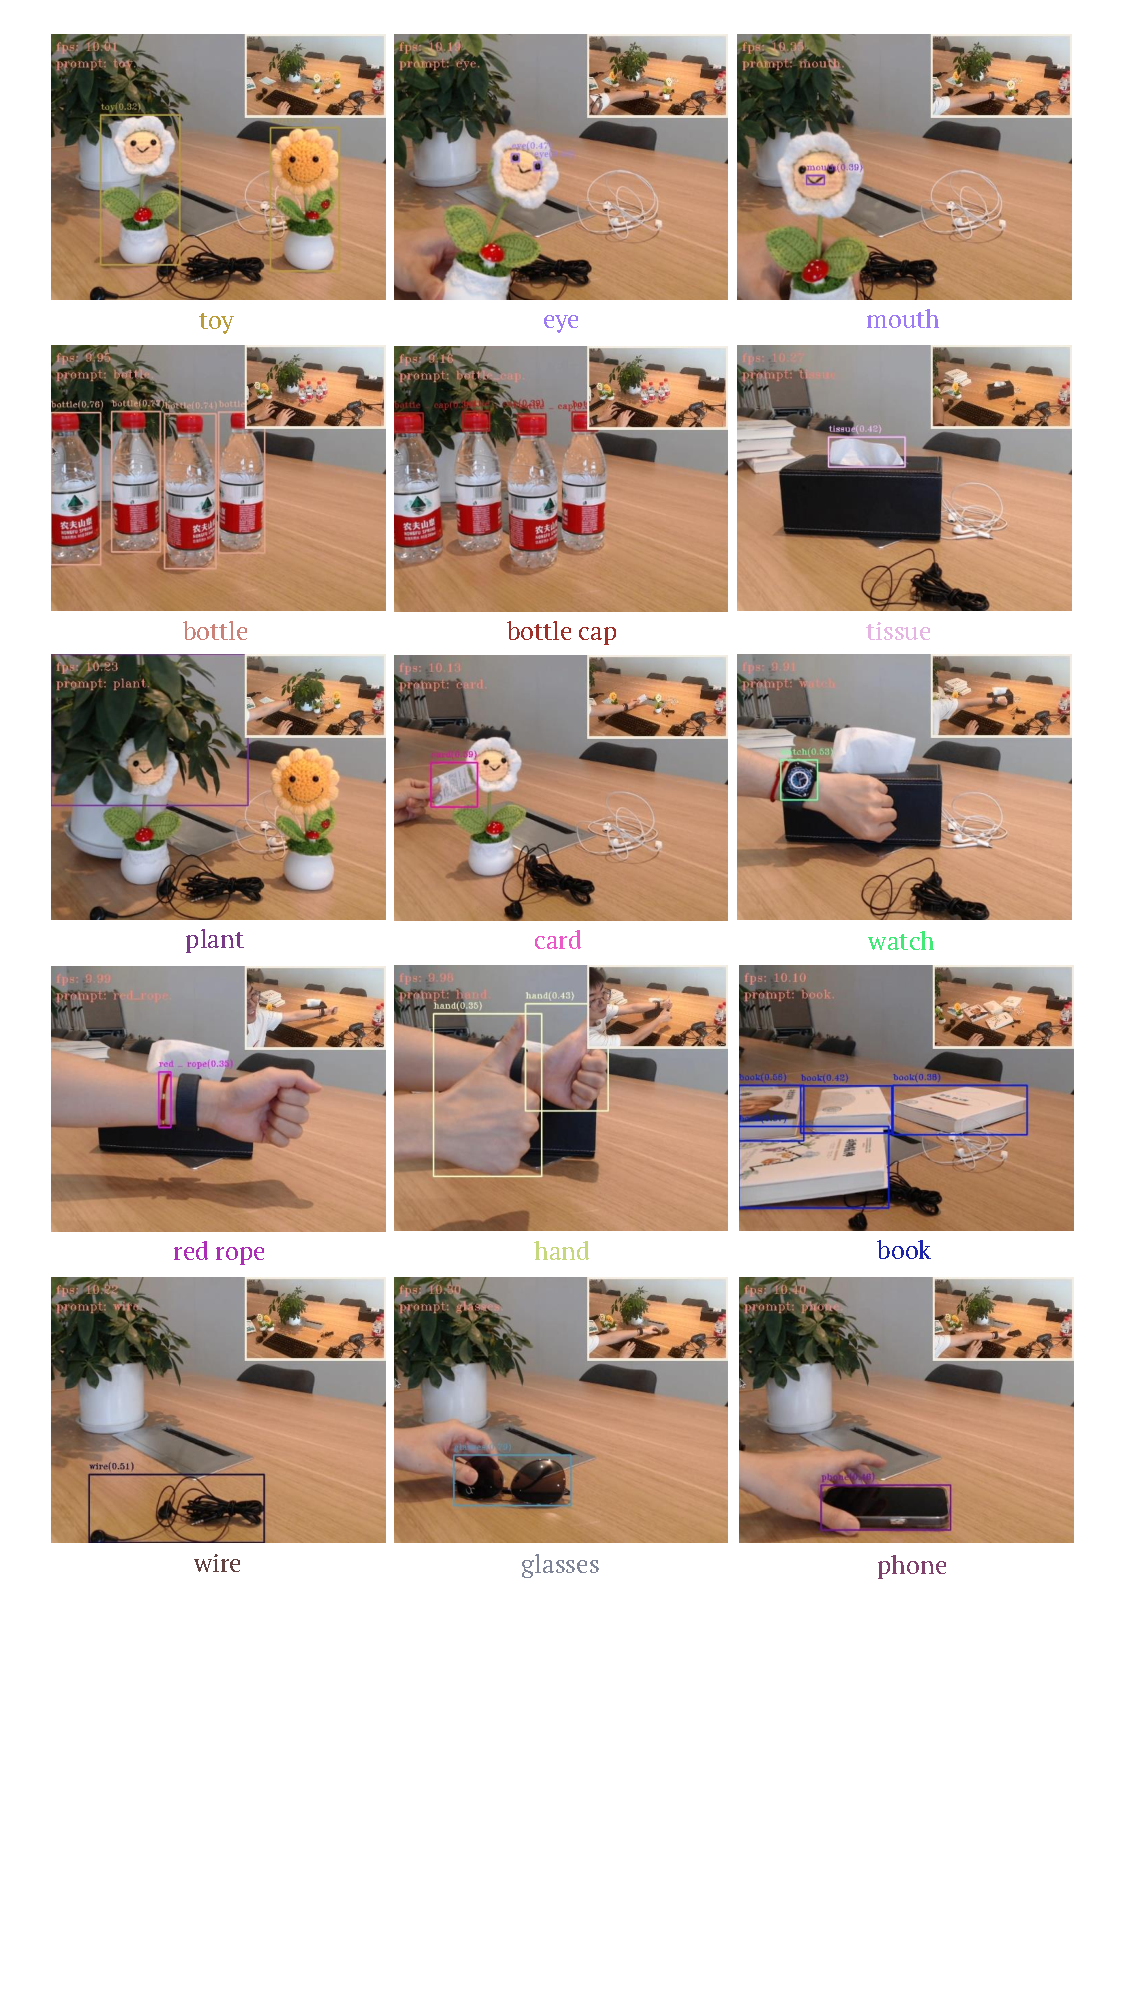
\includegraphics[width=\textwidth]{figs/edge_vis_v2.pdf}
    \caption{The visualization of Grounding DINO 1.5 Edge on NVIDIA Orin NX. The top left of the screen displays the FPS and prompts, while the top right shows a camera view of the recorded scene.}
    \label{fig:edge_vis}
    %\vspace{-4mm}
\end{figure}